%%%%%%%%%%%%%%%%%%%%%%%%%%%%%%%%%%%%%%%%%%%%%%%%%%%%%%%%%%%%%%%%%%%%%%%%%%%%%%%%
%2345678901234567890123456789012345678901234567890123456789012345678901234567890
%        1         2         3         4         5         6         7         8

\documentclass[letterpaper, 12 pt, conference]{ieeeconf}  % Comment this line out
                                                          % if you need a4paper
%\documentclass[a4paper, 12pt, conference]{ieeeconf}      % Use this line for a4
                                                          % paper

%\IEEEoverridecommandlockouts                              % This command is only
                                                          % needed if you want to
                                                          % use the \thanks command
%\overrideIEEEmargins
% See the \addtolength command later in the file to balance the column lengths
% on the last page of the document
\usepackage{graphicx}

\usepackage{hyperref}
\hypersetup{
    colorlinks=true,
    linkcolor=blue,
    filecolor=magenta,      
    urlcolor=cyan,
}

% The following packages can be found on http:\\www.ctan.org
%\usepackage{graphics} % for pdf, bitmapped graphics files
%\usepackage{epsfig} % for postscript graphics files
%\usepackage{mathptmx} % assumes new font selection scheme installed
%\usepackage{times} % assumes new font selection scheme installed
%\usepackage{amsmath} % assumes amsmath package installed
%\usepackage{amssymb}  % assumes amsmath package installed

\title{\LARGE \bf
Data Science Final Assignment B
}

%\author{ \parbox{3 in}{\centering Narshion Ngao*
%         \thanks{*Use the $\backslash$thanks command to put information here}\\
%         Msc. Computer Systems - 2018\\
%         Jomo Kenyatta University of Agriculture \& Technology \\
%       
%}}

\author{Renjie Zhou(rz296) \\% <-this % stops a space
Magdalene College
}


\begin{document}



\maketitle
\thispagestyle{empty}
\pagestyle{empty}


%%%%%%%%%%%%%%%%%%%%%%%%%%%%%%%%%%%%%%%%%%%%%%%%%%%%%%%%%%%%%%%%%%%%%%%%%%%%%%%%
\section{Data Preparation}
Since the data set used by this assignment is the original data set from DIABETES 130-US HOSPITALS FOR YEARS 1999-2008 DATA SET, which has about ten times the number of entries compared to that of the data set used in assignment A, they can potentially have different structure and distribution. Therefore, I re-examine the data set and pre-process the data based on the distribution of the original data set.\\
\newline
As the task is to predict the number of days between admission and discharge for the \textit{next visit} of each sample, I create a new attribute named  \textit{next\_time\_in\_hospital}. I first examined the number of encounters for each patient, and remove the samples with only one encounter from the data, as they do not have a value for  \textit{next\_time\_in\_hospital}. I then rearranged the encounters for each patient based on the chronological order of \textit{encounter\_id}. From there, it is easy to obtain the value for  \textit{next\_time\_in\_hospital} for each sample by taking  \textit{time\_in\_hospital} of the next encounter of the same patient. I then deleted the last encounter of each patient with multiple encounters in the data set, as these samples do not have a value for \textit{next\_time\_in\_hospital}. \\\newline
After processing to obtain \textit{next\_time\_in\_hospital}, I examined its distribution and its relation with age groups.\\
\begin{figure}[h]
  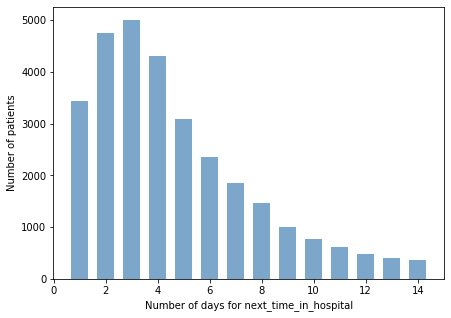
\includegraphics[width=9cm]{./figs/next_t.png}
  \caption{Number patients - number of days for next\_time\_in\_hospital}
  \label{fig:boat1}
\end{figure}
\begin{figure}[h]
  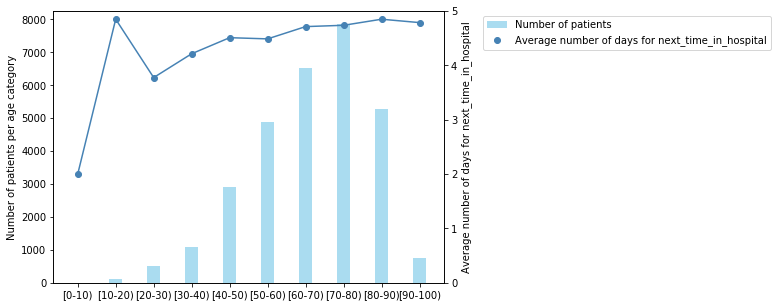
\includegraphics[width=10cm]{./figs/ave-ntih-inc-trd.png}
  \caption{Relation between number of patients and average number of next\_time\_in\_hospital per age group}
  \label{fig:boat1}
\end{figure}\newline
 From Fig 1, I can conclude that \textit{next\_time\_in\_hospital} has a normal distribution skewed towards left. This shows that most patients have fewer than 8 days for \textit{next\_time\_in\_hospital}. \\\newline
 There are two things that can be concluded from Fig 2 - first, the number of patients in the age group in the data set also has a normal distribution, but skewed towards right, which means that patients with higher ages have more encounters to the hospital; second, there are two parts in the line graph showing the average number of days for \textit{next\_time\_in\_hospital}: a sharp increase from age[0-10) to age[10-20), and then a more gentle increase from the younger to the older age groups. The interpretation is that as the age increases, it is more likely for the patient to revisit the hospital with longer stay, because with more people in the age group, the average number of days for next hospital visit should decrease if the number of days for each individual case remains roughly the same, however the trend shows the otherwise, hence the interpretation. \\\newline
 I also examined the relationship between readmission and the number of days for next visit to the hospital as shown in Fig 3 .\\
 \begin{figure}[h]
  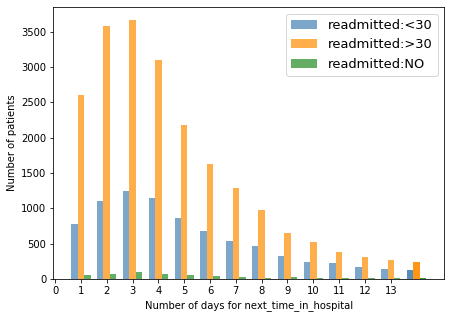
\includegraphics[width=8cm]{./figs/next_t_vs_rd.png}
  \caption{Relation between readmission and number of next\_time\_in\_hospital}
  \label{fig:boat1}
\end{figure}\newline
From the graph, the number of patients being readmitted after more than 30 days have a similar distribution as the number of days in the hospital for the next visit. This  means that despite many patients are readmitted after more than 30 days to inpatient visit, their time spent in the hospital for the next visit tend to be concentrated between 1 and 6 days instead of longer days. This might be because their conditions are not extremely severe, therefore they are admitted only after more than 30 days of impatient visits (but not fewer than 30 days), and their next time to stay after being readmitted is relatively short. Similarly, the patients readmitted with fewer than 30 days to inpatient visit may have more severe conditions, as the distribution of the days spent for next visit to hospital is more even compared to the group of patients with `readmitted $>$ 30', which means they tend to have longer stays for the next time of hospital visit.\\
\newline
 I then start pre-processing the data for training and testing.
 
\subsection{Missing values}
From assignment A, I know that some attributes in the data set have many missing entries, and some have very skewed distributions. Hence I start off by examining the attributes with a high percentage of missing values, namely `weight', `payer\_coder', `medical\_specialty'. I could have filled in missing values for `weight', however this will introduce much uncertainty, therefore I dropped the column from the data set. I dropped `payer\_code' as from the correlation matrix of the data set, `payer\_coder' has a very low correlation with `next\_time\_in\_hospital'. `Medical\_specialty' has a strong correlation with `next\_time\_in\_hospital'. Moreover, I was wondering whether the missing in the column have correlation with the outcome of interest, hence I filled the missing in with string `Missing', and hoped to draw more insights from further analysis. There are some missing values in primary, secondary and additional secondary diagnosis. I decided to drop them to avoid introducing too much uncertainty to the data.

\subsection{Attribute distributions, regrouping and filtering}
I then examined the distribution of each attribute in the data. 
\begin{figure}[h]
  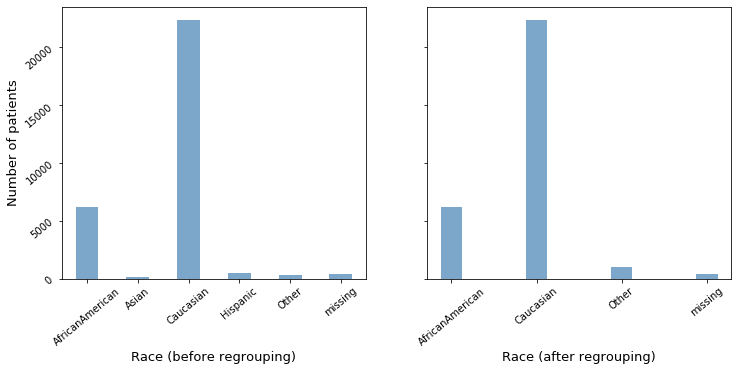
\includegraphics[width=9cm]{./figs/race_dist.png}
  \caption{Patient race distribution before (left) and after(right) regrouping}
  \label{fig:boat1}
\end{figure}\newline
Fig 4 shows that even with regrouping of the categories with very few samples for feature `race', there is still a very unbalanced distribution, which can lead to overfitting. Therefore I selected samples with `race' being Caucasian only, hoping to avoid the problem.\\\newline
\begin{figure}[h]
  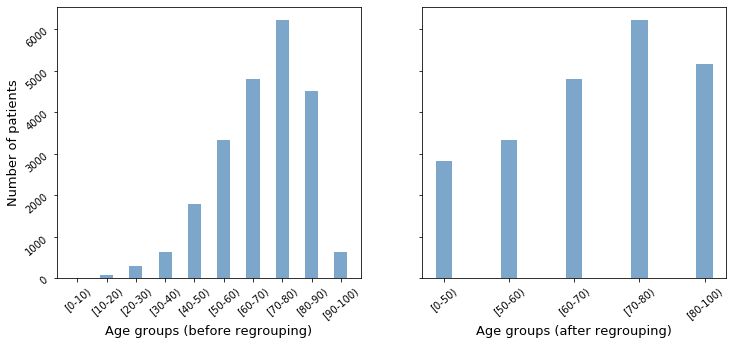
\includegraphics[width=9cm]{./figs/age_dist.png}
  \caption{Patient age group distribution before (left) and after(right) regrouping}
  \label{fig:boat1}
\end{figure}\newline
Fig 5 shows that regrouping of age groups shorten the tail of the distribution curve of age group, therefore reducing the possibility of overfitting for age group during training of the neural network.\\
\begin{figure}[h]
  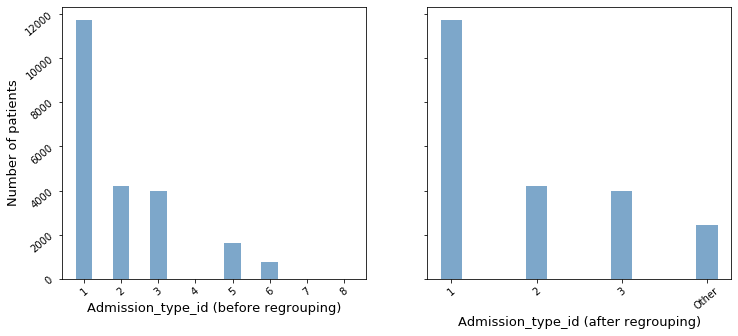
\includegraphics[width=8cm, height=4cm]{./figs/admin_type.png}
  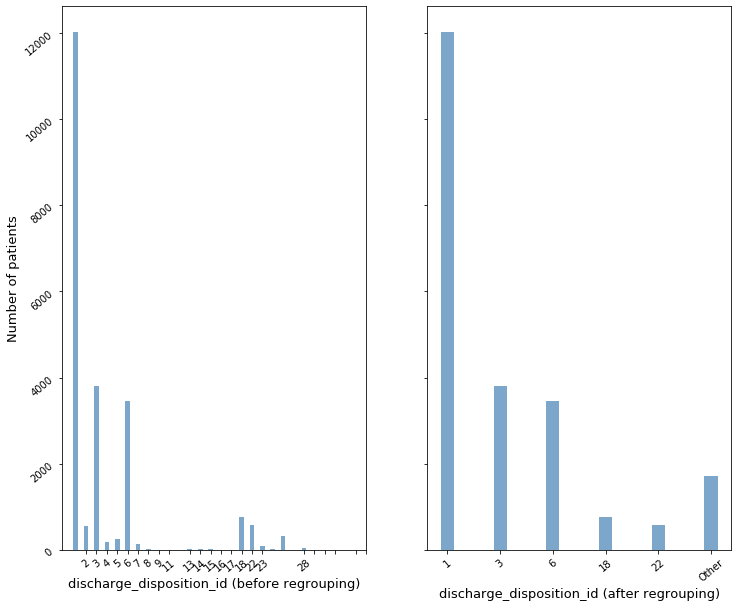
\includegraphics[width=8cm, height=4cm]{./figs/disc-pos.png}
  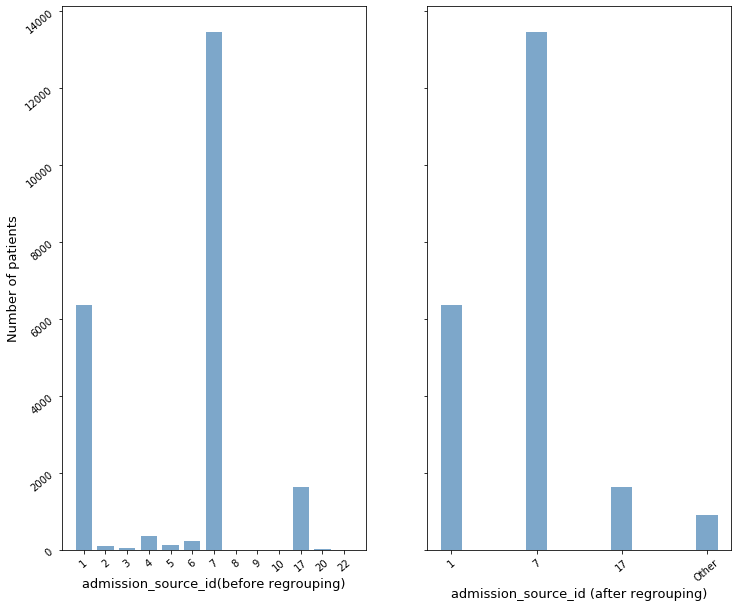
\includegraphics[width=8cm, height=4cm]{./figs/admis-source.png}
%  \caption{Patient distribution before (left) and after (right) grouping:\\(from 1st row to 3rd row) admission\_type, discharge\_position, admission\_source}
  \label{fig:boat1}
\end{figure}\newline
Similarly, Fig 6 shows that regrouping the categories for feature `admission\_type\_id' and `discharge\_disposition\_id', `admission\_source\_id' flatten the distribution curve and shorten the tail, which means that the samples are more evenly distributed across different categories for each attribute mentioned above. This can reduce the possibility of overfitting during training, therefore potentially improving the results.\\
\newline
For feature `medical\_specialty', `diag\_1', `diag\_2' and `diag\_3', there are many categories with only handful of  cases as well, potentially resulting in overfitting. I regrouped them based on table describing the textual categories of medical specialties and different diagnoses instead of using the numerical format of the labels. I left the remaining features untouched as their values are either binary in nature, or have numerical meaning to mark certain bench marks, which should not be changed.\\\newline
After pre-processing, the final data set that I used for training has 22346 samples with 239 features excluding \textit{next\_time\_in\_hospital}, with both numerical attributes and categorical attributes. Numerical attributes are `time\_in\_hospital', `num\_procedures', `num\_medications', `number\_outpatient', `number\_emergency', `number\_inpatient', `number\_diagnoses', whereas the rest of features are categorical. `number\_lab\_procedures' has been dropped as it does not show a strong correlation with the outcome of interest.\\\newline
Finally, I have scaled the data using max-min scaling to ensure that all data fall between 0 and 1. I used Max-min scaling instead of standard scaling because it is more intuitive to me to have all values between 0 and 1 when there are categorical attributes encoded using one-hot encoding.
\subsection{Data splitting}
\begin{figure}[h]
  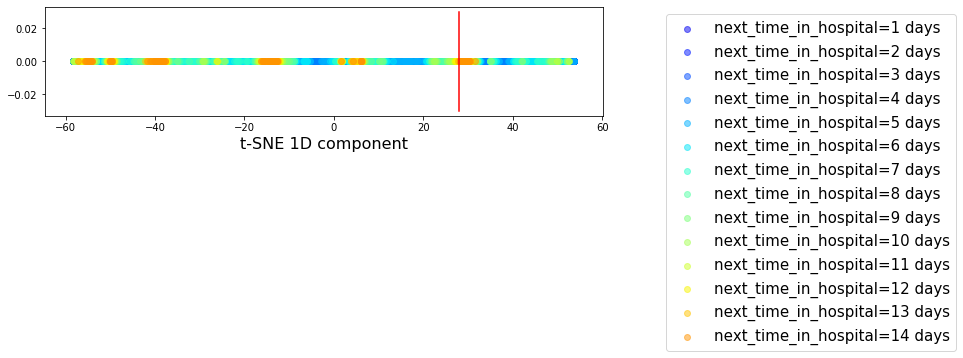
\includegraphics[width=9cm]{./figs/tSNE_split.png}
  \caption{Dimensionality reduction to 1D of all sample points}
  \label{fig:boat1}
\end{figure}
Since I want to generalise the final result, instead of using stratified sampling, I applied t-SNE dimensionality-reduction technique to reduce all samples down to 1D, and select the 20\% data points on the rightmost end of the number line, as illustrated in Fig 7, where all points on the left of the red line belong to training set, and the rest testing set. This gives a general division between the data points, because t-SNE clusters the data points on 1-dimensional space by throwing all points along a number line first, and grouping them together by using the probability distribution to model the similarity of points. Hence, t-SNE preserves the original structure of the data in high dimensionality in low dimensionality, and samples that are close to each other in the original space will cluster together along the number line in 1-D space as well. As such, the top 20\% of data point of the right end of the number line are most likely close to each other in the original space. \\\newline 
Furthermore, I coloured the points using values of \textit{ next\_time\_in\_hospital}, and the mix of color along the entire line shows that in the training and testing sets, there is a balanced coverage of all values of the target, ensuring a balanced split.

%%%%%%%%%%%%%%%%%%%%%%%%%%%%%%%%%%%%%%%%%%%%%%%%%%%%%%%%%%%%%%%%%%%%%%%%%%%%%%%%
\section{Loss function}
A loss function is the function that will be minimised during the training of the Neural Network architecture (NN). As the task in this assignment is a regression task which aims to predict number of days for the next visit, given the mean value of the number of days calculated from the true values of the target, it is plausible to derive the loss function from the Poisson distribution, which can be used to model the rate parameter of the occurrence. However, Poisson distribution has two assumptions - a constant mean rate and occurrences being independent from each other. The former one can be assured as the given data has a limited number of samples with given values for the target, hence a constant mean can be calculated from it; the later one may not hold in reality, since the number of days for a sample's next visit may be dependent on it's previous visit, since the values come from the same patient. \\\newline
Nevertheless, assuming that the both assumptions hold in this case, I chose to use the Poisson distribution to model the number of days for next hospital visit. \\\newline
Given the mathematical formula of Poisson distribution:
\begin{center}
$P\left(X= x \right) = \frac{{e^{ - \lambda } \lambda ^x }}{{x!}}$    
\end{center}
where X in this case is the random variable of number of days for next visit in the hospital, x is the number of days for the next visit that we want to know the probability of occurrence, and $\lambda$ is the mean value of X, here, the mean number of days of visit across all samples, I want to derive a function which, when decreasing, increases the actual probability $P\left(X= x \right)$. This can be achieved by rearranging the original formula and taking logarithm. The final form of the loss function is then:
\begin{center}
    $L(y, \hat{y}) = \sum_{i=0}^{N}\hat{y_i} - y_i log \hat{y_i}$
\end{center}
where \textit{y} is the true target values, and $\hat{y}$ is the predicted target values.

\section{Machine learning algorithms implementation}
\subsection{Model and Design Choices}
I decided to implement a Multilayer-Perceptron NN to perform this regression task. MLP is a popular simple NN architecture that can be felxibly tailored to perform either classification or regression task as needed, to map inputs to an output. In this case, I implemented the model to perform a regression task by only having one unit on the output layer. \\\newline
There are numerous variations that I need to control and investigate to construct an optimal MLP. In this case, I have looked into learning rate of the mode, number of neurons in each layer, drop out rate on each drop out layer and the activation function used in each layer.
\\
\subsubsection{Learning rate}
Learning rate determines how big a step the model changes for each step, and therefore is critical to the final learning performance of the model. I have set the learning rate relatively small for different variations, as the data set is not very big, hence having big learning rate may not converge eventually. 
\\
\subsubsection{Number of neurons per layer}
Number of neurons determines how many values to store internally on each layer. It affects the results of matrix multiplication during the training, and therefore should be selected carefully with multiple trials.
\\
\subsubsection{Drop out rate}
As the data set contains some missing values and is potentially noisy, I added drop out layer for each MLP model to reduce any chance of overfitting by performing regularisation. Drop out rate affects the strength of regularisation, and hence should be selected carefully. For the sake of comparison, I selected drop out rate=0 as one of the values for variations.
\\
\subsubsection{Activation function}
Activation function determine the output of a neural network by determining whether the output of each neuron should be passed down to the next level. Hence it is highly influential in determining the final output values. I have selected  rectified linear unit ('ReLU') and tanh function for the variations as they are very popular and commonly used in NNs in many papers.\\

Epoch is the number of iterations that MLP runs on the data to fine tune the parameters, where as batch size is the number of samples processed by MLP before updating the parameters. Due to time constraints, I have set batch size = 10 for MLPs with both 0 and 1 hidden layer, and set epoch = 30 for MLPs with 0 hidden layer and epoch = 20 for MLPs with 1 hidden layer.\\
\newline
Due to time constraint, I have selected `Adam' as the only variation for the optimizer of the model, as it is claimed to have good performance based on other papers.\\\newline
In order to investigate the impact of different parameters on the two metrics - accuracy and training time, I have tweaked variations to construct various MLPs and ran them on the prepared data. The tables below shows the list of parameters that I have tweaked, and for each, a list of values that I have tried with, with 0 and 1 hidden layer respectively.  
\begin{center}
 \begin{tabular}{||c| c||} 
 \hline
 learning\_rate &  [0.0001, 0.0005, 0.001, 0.003]\\
 \hline
 num of neurons & [128, 256, 512] \\
 \hline
 dropout rate & [0.0, 0.2, 0.5]\\
 \hline
 activation function & [ReLU, Tanh]\\ 
 \hline
\end{tabular}
Table 1: Parameters and values for MLP with 0 hidden layer
\end{center}
After trying different parameters for MLP with 0 hidden layer, I have concluded that for this specific data set, MLP with 0 hidden layer has the best accuracy with learning rate = 0.0005, number of neurons for the input layer = 128, dropout rate = 0.5 and activation function = ReLu. Due to time constraint, I have fixed the number of neurons to be 128 and the drop out rate for the first drop out layer to be 0.5 when constructing the MLPs with 1 hidden layer. \\
\begin{center}
 \begin{tabular}{||c| c||} 
 \hline
 learning\_rate &  [0.0001, 0.0005, 0.001, 0.003]\\
 \hline
 num of neurons & [32, 64, 128] \\
 \hline
 dropout rate & [0.0, 0.2, 0.5]\\
 \hline
 activation function & [ReLU, Tanh]\\ 
 \hline
\end{tabular}
Table 2: Parameters and values for MLP with 1 hidden layer
\end{center}
The number of neurons and the drop out rate in Table 2 refer to that of the hidden layer and the second drop out layer respectively. 
\subsection{Dimensionality Reduction using PCA}
To investigate whether dimensionality reduction has an impact on the accuracy level of the prediction and the training time, I applied PCA to reduce the dimensionality of the processed data set before training the models on it. I selected the best performed models, one with 0 hidden layer and the other with 1 hidden layer, and ran them on PCA-reduced data set. I have tried various numbers of principle components (PCs) ranged from 10 to 50 with a step of 10 PCs. 
\subsection{Results and interpretations}
The two tables below demonstrate the parameters of the two best performed MLPs:\\
\begin{center}
 \begin{tabular}{||c| c||} 
 \hline
 learning\_rate &  0.0005\\
 \hline
 num of neurons & 128 \\
 \hline
 dropout rate & 0.5\\
 \hline
 activation function & ReLU\\ 
   \hline
epoch & 30\\ 
 \hline
 batch size & 10\\ 
 \hline
 test accuracy & 0.13152\\
 \hline
\end{tabular}\\
Table 3: Parameters values for best-performed MLP with  0 hidden layer
\end{center}
\begin{center}
 \begin{tabular}{||c| c||} 
 \hline
 learning\_rate &  0.0001\\
 \hline
 first num of neurons & 128 \\
 \hline
  first dropout rate & 0.5\\
 \hline
 second num of neurons & 32 \\
 \hline
 second dropout rate & 0.0\\
 \hline
 activation function & ReLU\\ 
  \hline
epoch & 20\\ 
 \hline
 batch size & 10\\ 
 \hline
 test accuracy & 0.14940\\
 \hline
\end{tabular}\\
Table 4: Parameters values for best-performed MLP with  1 hidden layer
\end{center}
From the table above, it shows that MLP with 1 hidden layer performs better than that with only 0 hidden layer. This means that having one hidden layer helps with learning even when using the same activation function and optimizer. The number of neurons in the second layer shown in Table 4 is much fewer than that in the first layer, and the drop out rate of the second drop out layer shown in the Table 4 is 0. The interpretation is that with a much smaller number of neurons and lower drop out rate after the input layer and the first drop out layer, the model tends not to overfit, resulting in a higher accuracy.\\\newline
However, one thing to be noticed is that even the accuracy of the best performed MLP is exceptionally low for this task. This may be because of not enough depth for the model, as there is only one hidden layer, or not appropriate activation function, as I did not have a very wide range of choices for activation function. Furthermore, it may even show that MLP is not suitable for performing a regression task and I should try other models for such task instead.

\subsection{Measurement}
\subsubsection{Original dataset}
Apart from selecting the best model to perform the regression task, another aim is to measure the training time of different models based on variations. The change in time can be shown in the Fig 7 below (next page), with variations in the parameters described above. By observing each graph, we can conclude that for a given number of hidden layer in the MLP, at a given number of neurons for the input layer, both an increase in the drop out rate and an increase in the learning rate increase the time taken for the training. By observing the y axes, we can conclude that increasing the number of neurons for each layer increases the training time regardless of any increase in other parameters. Also, by comparing the y axes of the graphs for using ReLU and using Tanh activation function, we can conclude that training time is overall shorter when using ReLU activation function than using Tanh activation function. This can be explained by simpler mathematical formula of ReLU activation compared to Tanh, as ReLU is just selecting positive output values, and replacing the negative ones with zeros.
\begin{figure*}[h]
	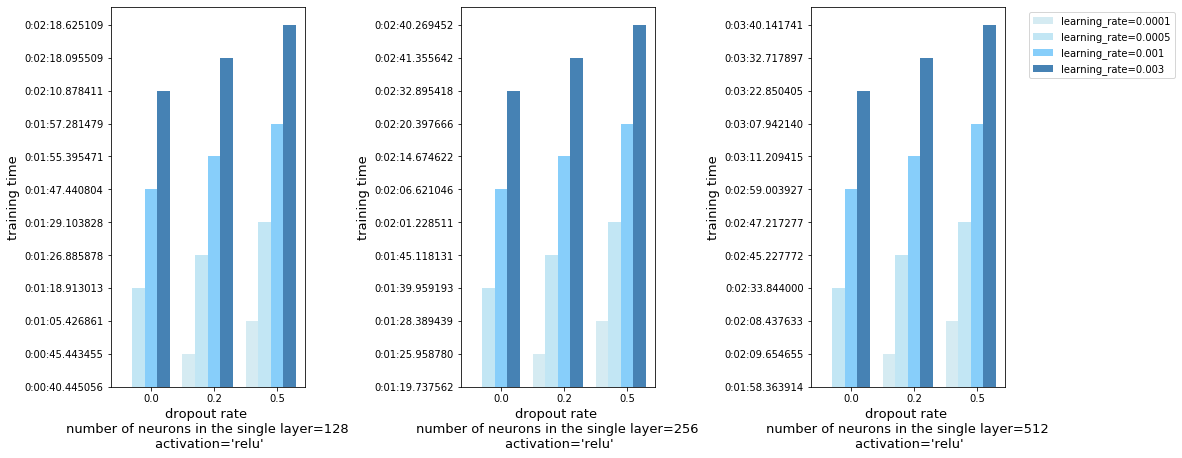
\includegraphics[width=18cm, height=5cm]{./figs/time-relu.png}\\
		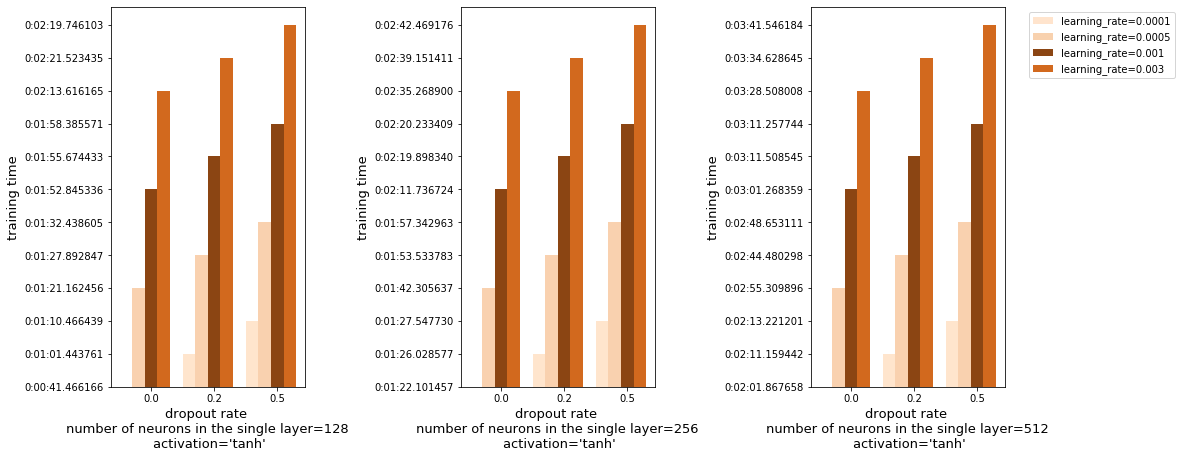
\includegraphics[width=18cm, height=5cm]{./figs/time-tanh-layer1.png}
	\caption{Time - drop out rate using different activation for MLP with 0 hidden layer}
	\label{fig:boat1}
\end{figure*}\\
Fig 8 shows similar graphs of time vs drop out rate for different variations of the parameters for training MLP with 1 hidden layer. By observing the y axes, I obtain the same conclusion as the ones from the graph for MLP with 0 hidden layer. Overall, by comparing the y axes of Fig 7 and Fig 8, it can be concluded that MLP with more hidden layers have longer training time. Also, from the same shape of each graph, it shows that an increase in the drop-out rate results in the same proportion of increase in time regardless of other parameters.\\
\begin{figure*}[h]
	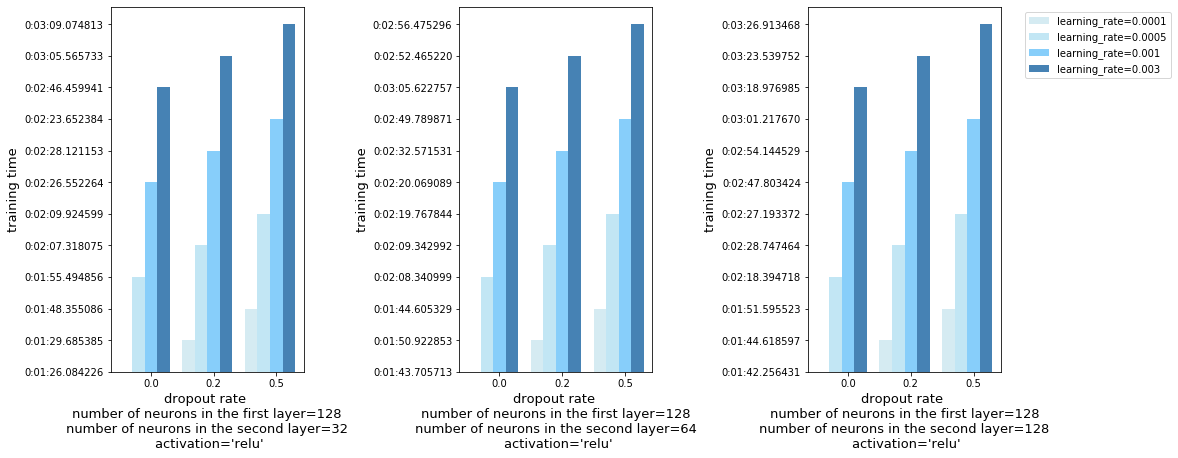
\includegraphics[width=18cm, height=5cm]{./figs/2-layers-time-relu.png}\\
	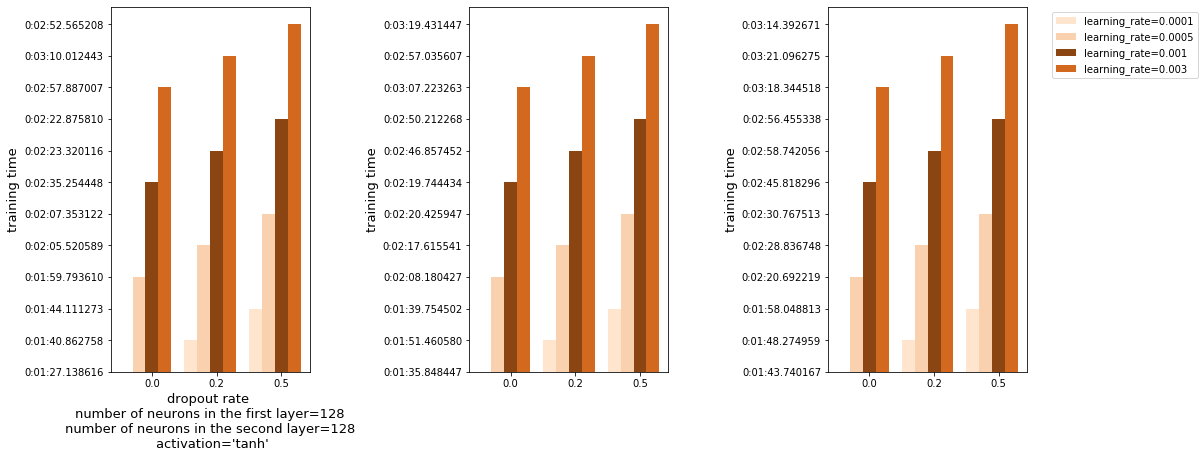
\includegraphics[width=18cm, height=5cm]{./figs/time-tanh.png}
	\caption{Time - drop out rate using different activation for MLP with 1 hidden layer}
	\label{fig:boat1}
\end{figure*}\\

\subsubsection{PCA-reduced dataset}
Given the time constraint, I have performed PCA dimensionality reduction with n\_components = [10, 20, 30, 40, 50], and applied the best formed model, MLP, with 1 hidden layer and the fine tuned parameters. Fig 9 shows the training time for MLPs on each number of components in the range selected. From the plot, it shows that with a reduced number of features, the training time decreases from 1 minute 55.4948 seconds to the time ranged from 32.8915 seconds to 36.8438 seconds. This is a 70.6\% decrese from the original training time.\\
\begin{figure}[h]
	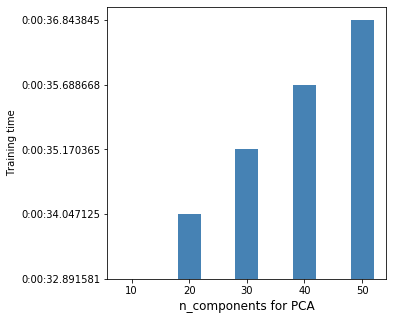
\includegraphics[width=8cm, height=6cm]{./figs/pca_t.png}\\
	\caption{Training time for data reduced by PCA}
	\label{fig:boat1}
\end{figure}\\
\section{Evaluation}
Finally, I have chosen the two best performed models to evaluate their performances. Fig 10 and 11 below shows the accuracy and loss during the training process.\\
\begin{figure}[h]
	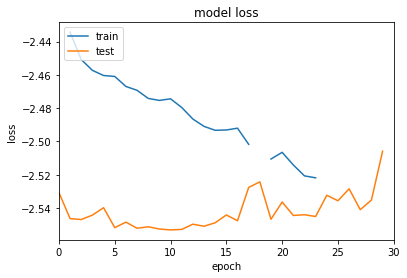
\includegraphics[width=8cm, height=4cm]{./figs/mlp-loss_1.png}\\
	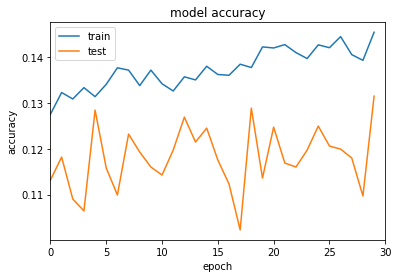
\includegraphics[width=8cm, height=4cm]{./figs/mlp-accuracy_1.png}
	\caption{Time - Performance of MLP with 0 hidden layer}
	\label{fig:boat1}
\end{figure}\\
\begin{figure}[h]
	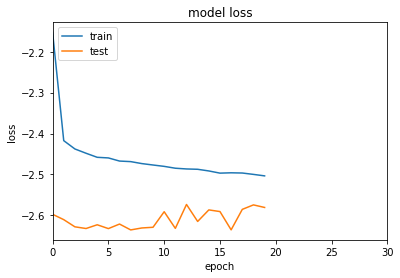
\includegraphics[width=8cm, height=4cm]{./figs/mlp-loss_2.png}\\
	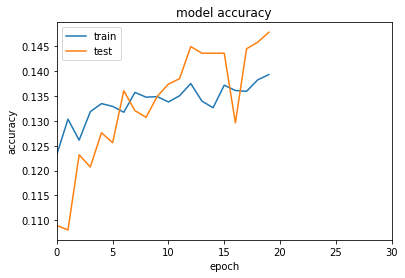
\includegraphics[width=8cm, height=4cm]{./figs/mlp-accuracy_2.png}
	\caption{Time - Performance of MLP with 1 hidden layer}
	\label{fig:boat1}
\end{figure}\\
This shows a better performance of the MLP with 1 hidden layer, even when the number of epoch is smaller (20 epochs) than that for training MLP with 0 hidden layer (30 epochs).  The line for test accuracy in Fig 10 fluctuates much more than that of training accuracy, compared to the line for testing set in Fig 11, which may explain the poorer performance of MLP with 0 hidden layer than MLP with 1 hidden layer for the testing set. Additionally, from the plots in the two loss graph, it also shows that MLP with 1 hidden layer minimises the loss function better for testing set compared to MLP with 0 hidden layer. However, one interesting thing to note is that MLP with 2 hidden layer perform worse on training set than testing set. \\\newline
With PCA, the accuracy level increases further from the best performance available. Fig 12 shows the accuracy and loss plot of the model when training using the 20 PCs, which gives the best accuracy among all models trained using different number of PCs. The accuracy increases from 0.14940 to 0.16577. This may be explained by that using the top 20 PCs for training reduces the noise level in the data, and also covers the most important features. Use a data set with lower dimensionality also helps reducing the possibility of overfitting.\\\newline
However, even with PCA, the accuracy level is still fairly low. The prediction is about $\pm3$ days away from the target values. 
\begin{figure}[h]
	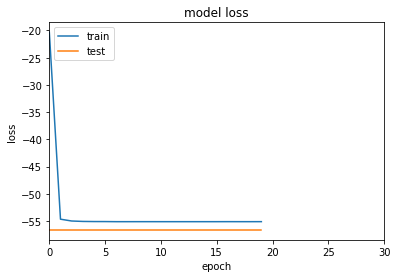
\includegraphics[width=8cm, height=4cm]{./figs/mlp-loss_20.png}\\
		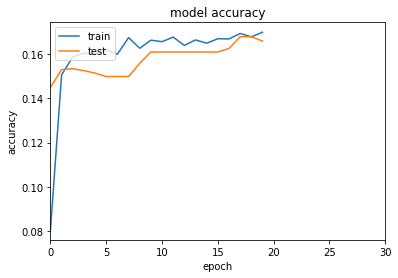
\includegraphics[width=8cm, height=4cm]{./figs/mlp-accuracy_20.png}\\
	\caption{Time - Performance of MLP with 1 hidden layer on 20 PCs of the data}
	\label{fig:boat1}
\end{figure}\\

\section{Conclusion}
Since the data set is split in the way that can probably give a reasonable indication of the prediction accuracy in novel scenarios, I believe that the best MLP predictor obtained in this report can perform the regression task with similar performance level in the novel scenarios. However, since the accuracy is very low, the more essential conclusion drawn from the report might be training an MLP with deeper layers or not using MLP for such task, but looking for a model with better performance. In terms of measurement of training time, I believe that the smaller values for various parameters lead to a shorter training time, and the dimensionality reduction using PCA leads to a significantly reduced training time.
\end{document}